\documentclass[10pt,journal,compsoc]{IEEEtran}
\usepackage{kotex}
\usepackage[utf8]{inputenc}
\usepackage{graphicx}
\usepackage{cleveref}

\ifCLASSOPTIONcompsoc

  \usepackage[nocompress]{cite}
\else

  \usepackage{cite}
\fi

\ifCLASSINFOpdf

\else

\fi

\hyphenation{op-tical net-works semi-conduc-tor}


\begin{document}

\title{k-means를 이용한 인구 밀집지역 분포도 형성 및 분석}

\author{Cheol~Woo~Park,~\IEEEmembership{}
        Jun~Young~Park.~\IEEEmembership{}
       
\IEEEcompsocitemizethanks{\IEEEcompsocthanksitem Cheol~Woo~Park was with the Department
of Electronics Engineering, Pusan National University, 2 Busandaehak-Ro 63 Beon-Gil, Pusan 46241, Republic of Korea.\protect\\
E-mail: cwoop92@pusan.ac.kr

\IEEEcompsocthanksitem Jun~Young~Park was with the Department
of Electronics Engineering, Pusan National University, 2 Busandaehak-Ro 63 Beon-Gil, Pusan 46241, Republic of Korea.\protect\\
E-mail: jyp1324236@naver}
\thanks{}}

\markboth{}%
{Shell \MakeLowercase{\textit{et al.}}: Bare Demo of IEEEtran.cls for Computer Science Journals}

\IEEEtitleabstractindextext{%
\begin{abstract}
코로나19 바이러스 확진자가 점차 늘어나면서 그 기세가 쉽게 꺾이지 않을 것으로 보인다. 본 보고서에서는 주요 통행 패턴을 분석하여 효과적인 방역지점 선정 및 운용 방안을 제안하고자 한다. 먼저 T-Drive trajectory data sample을 DBSCAN을 이용하여 데이터들을 전처리 한 뒤, k-means clustering 알고리즘을 이용하여 시민들이 자주 방문하는 거점들을 분류하는 방법을 제안한다. 본 보고서는 시민들의 통행 경로를 분석하여, 장기화되고 있는 코로나19 사태 속에서 감염 확산을 효과적으로 막기 위한 안전 통행 경로 운용에 관해서 제안했다.
\end{abstract}

% Note that keywords are not normally used for peerreview papers.
\begin{IEEEkeywords}
Computer Science, covid-19, k-means.
\end{IEEEkeywords}}


% make the title area
\maketitle


% To allow for easy dual compilation without having to reenter the
% abstract/keywords data, the \IEEEtitleabstractindextext text will
% not be used in maketitle, but will appear (i.e., to be "transported")
% here as \IEEEdisplaynontitleabstractindextext when the compsoc 
% or transmag modes are not selected <OR> if conference mode is selected 
% - because all conference papers position the abstract like regular
% papers do.
\IEEEdisplaynontitleabstractindextext
% \IEEEdisplaynontitleabstractindextext has no effect when using
% compsoc or transmag under a non-conference mode.



% For peer review papers, you can put extra information on the cover
% page as needed:
% \ifCLASSOPTIONpeerreview
% \begin{center} \bfseries EDICS Category: 3-BBND \end{center}
% \fi
%
% For peerreview papers, this IEEEtran command inserts a page break and
% creates the second title. It will be ignored for other modes.
\IEEEpeerreviewmaketitle



\IEEEraisesectionheading{\section{Introduction}\label{sec:introduction}}
% Computer Society journal (but not conference!) papers do something unusual
% with the very first section heading (almost always called "Introduction").
% They place it ABOVE the main text! IEEEtran.cls does not automatically do
% this for you, but you can achieve this effect with the provided
% \IEEEraisesectionheading{} command. Note the need to keep any \label that
% is to refer to the section immediately after \section in the above as
% \IEEEraisesectionheading puts \section within a raised box.




% The very first letter is a 2 line initial drop letter followed
% by the rest of the first word in caps (small caps for compsoc).
% 
% form to use if the first word consists of a single letter:
% \IEEEPARstart{A}{demo} file is ....
% 
% form to use if you need the single drop letter followed by
% normal text (unknown if ever used by the IEEE):
% \IEEEPARstart{A}{}demo file is ....
% 
% Some journals put the first two words in caps:
% \IEEEPARstart{T}{his demo} file is ....
% 
% Here we have the typical use of a "T" for an initial drop letter
% and "HIS" in caps to complete the first word.
\IEEEPARstart{2}019년 12월 중국 우한 지역으로부터 시작된 코로나19 바이러스는 2020년 1월 23일 중국 교통의 중심지인 우한 지역 봉쇄라는 초유의 사태를 낳으며, 전 세계로 급격하게 전파되었다. 코로나의 확산은 치료제도 없는 상태에서 엄청난 속도로 계속하여 퍼져나가자, 세계 보건기구 WHO는 1968년 홍콩독감과, 2009년 신종플루를 제외하고는 선언한 적이없는 펜데믹사태를 선언하였다. 한국의 경우, 1월 20일 인천지역에서 발생한 최초 감염자를 시작으로 2월 21일부터 급속하게 증가하여, 7월 2일 현재 사망자 282명, 확진자 12,904명에 육박하고 있으며, 세계적으로 사망자 514,107명, 확진자 10,578,973명에 육박하였다.또한 현재 미국에서는 연 이틀 동안 15만명 이라는 엄청난 사람 수의 확진자가 나오면서 제 2의 팬데믹 사태에 직면해있다. 그 기세가 쉽게 꺾이지 않을 것으로 보인다.

특히, 일부 환자의 경우 감염 이후 확진 판정 전까지 지역사회를 활발하게 이동·활동하면서 다수의 접촉자와 2차 감염자를 유발하고 있는 실정이다. 대구 경북 지역에서 2월 18일 확진 판정을 받은 환자의 경우, 2월 10일부터 고열과 폐렴 증상을 보이며 바이러스 의심을 받았으나, 병원의 지속적인 검사 제안을 거부한 채, 일주일 동안 500명가량이 참석하는 종교 예배, 결혼 예식장, 호텔 등을 돌며 다수의 접촉자와 감염자를 유발하였다. 또한, 시시각각 해외에서 입국하는 사람들과 특정 대규모 종교 활동에 참석한 다수의 접촉자와 의심 환자들의 신원과 행방을 초기에 파악하지 못하면서 급속한 지역 감염의 불씨가 되었다.

이러한 바이러스의 급속한 전파를 차단하기 위해서 시민들이 모여있을 장소를 예측하여 미리 경고, 방역하는 것이 중요하고, 빅데이터를 수집 및 분석해 코로나에 대비하는 연구가 각광을 받고 있다. 빅데이터는 문자 그대로 방대한 양의 데이터를 의미하는 것으로 빅데이터 분석은 과거의 현상 및 사실을 통해서 앞으로 미래에 이와 유사한 형태의 결과가 나타날 것이라는 가정으로 시작한다.

 빅데이터가 최근에 주목을 받는 이유는 크게 두가지로 정리할 수 있는데, 첫번째로 인터넷과 스마트폰의 등장으로 소셜 네트워크 서비스 등을 통해 언론매체가 아닌 개인이 정보를 유통할 수 있게 되어, 활용할 수 있는 데이터 양이 급격하게 증가하였고, 두번째로는 저장 비용의 감소로 인하여 클라우드 서비스가 더욱 보편화 되어, 데이터 처리기술이 비약적으로 발전해 데이터 처리 속도가 빨라졌기 때문이다.
 
 빅데이터를 통해 미래를 예측하는 대표적인 사례는 구글의 독감 예보 서비스를 들 수 있다. 2007년 구글에서는 일정기간의 검색어 분석을 통해 독감 유형의 패턴과 독감 발생 가능성이 높은 지역을 예측하는 독감 예보 서비스를 시작하였다. 이 서비스는 독감에 대한 증세나 호전방법, 약품 등의 검색 등과 같은 검색어를 분석함을 써 예측이 이루어진다. 이는 독감과 인터넷 검색어 빈도수와 같이 서로 직접적인 관계가 없어 보이는 요소가 실제 미래 예측에서 어떻게 반영될 수 있는지를 잘 보여주는 예이다. 이 서비스를 통해 구글은 2009년 2월 대서양 연안 중부지역의 주에서 감기가 확산될 것이라고 예측했는데, 이는 미국의 질병통제예방센터보다도 2주나 먼저 예측하여 구글 독감 트렌드가 더욱 이목을 받게 되는 계기가 되었다. 더불어 구글은 질병통제예방센터의 보고서보다 1~2주 빨리 독감 바이러스 활성을 예측하는 실시간 감지 시스템에 대한 컴퓨터 모델을 제시하였고, 그 결과를 세계적인 학술지인 네이처에 게재하기도 하였다.
 
본 보고서에서는 시민들이 군집 될 장소를 예측하기 위해, 코로나가 일어나기 전 T-Drive trajectory data sample를 이용하여 시민들의 통행 경로를 분석해 주요 통행 패턴을 분석, 현재에 효과적인 방역 지점 선정 및 운용 방안을 제안하고자 한다.

\begin{figure*}[htp] 
    \centering
    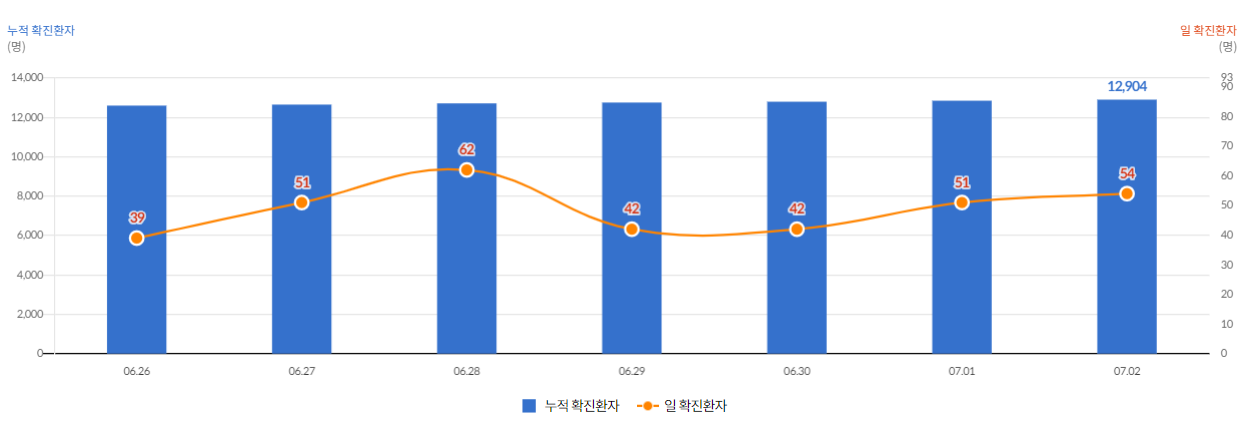
\includegraphics[width=\textwidth]{1.png} 
    \caption{국내 일일 및 누적 확진환자 추세} 
    \label{fig:1} 
\end{figure*}

\begin{figure*}[htp] 
    \centering
    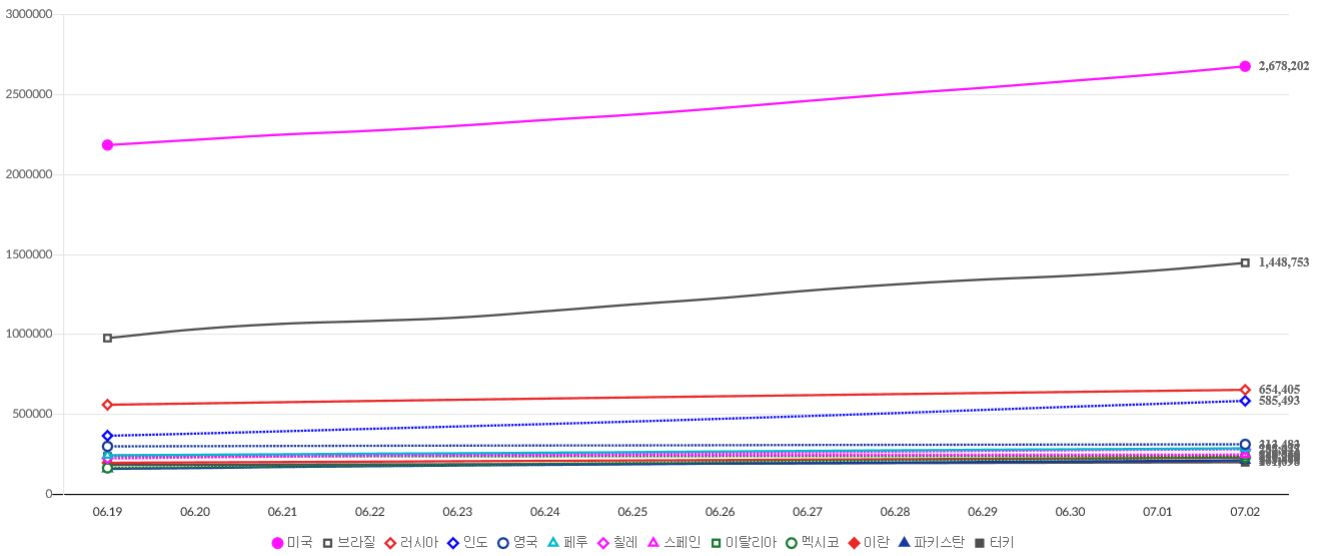
\includegraphics[width=\textwidth]{4.jpg} 
    \caption{누적발생 20만 이상 국가 발생 현황} 
    \label{fig:2} 
\end{figure*}

\section{The problem}

장기화되고 있는 바이러스의 지역 확산을 효과적으로 차단 및 관리하기 위해서는 효과적인 방역 지점을 선정하여 운영하고 시민들의 안전을 도모할 수 있는 안전 운행 경로 운용 등 효율적인 관리방안이 필요하다.
 
먼저 시간대별로 구축된 통행 사슬 DB를 이용하면,
시민들이 밀집된 지역을 중심으로 주요 통행 패턴과 경로를 파악할 수 있으며, 이러한 통행 패턴 정보를 활용하면, 장기화 되고 광역화 되고 있는 지역 감염 확산 속에서 제한 된 방역 자원을 효율적으로 운용할 수 있는 시간대별 방역 지점을 효과적으로 선정할 수 있다. 또한, 시민들이 많이 군집하는 지역의 시간대별 통행 및 혼잡 패턴을 분석하여, 시민의 불편을 최소화 하고 안전을 최대한 도모할 수 있는 안전 통행 경로 정보를 제공 및 운용할 수 있을 것이다. 마지막으로 바이러스 확산으로 인하여 변화된 통행 패턴을 고려한 대중교통 노선 및 스케쥴을 조정하고 이에 따른 다양한 교통 운영 전략을 마련할 수 있을 것이다.

정보통신기술의 발달과 스마트폰, 내비게이션 등의 개인 IT 장비가 지속적으로 확대되면서, 사람, 차량, 대중교통 이용자의 통행을 분석할 수 있는 모빌리티 빅데이터가 구축되었다. 이러한 모바일 통신, 대중교통카드, 차량 내비게이션 자료를 활용하면 개별 이동 경로는 물론, 통행 수단과 목적까지 파악할 수 있는 개인 통행 사슬 DB를 구축할 수 있다. 

그 중 T-Drive trajectory data sample는 택시의 내비게이션 단말기나 핸드폰 애플리케이션을 통해서 매초 기록되는 차량의 이동 궤적 정보이다. T-Drive trajectory data sample을 이용하면, 각 택시의 이동 및 위치를 지속적으로 기록하기 때문에 토지 이용 정보와 함께 통행 패턴을 분석하여, 사람들이 빈번하게 통행하는 지점을 찾는 것이 핵심 목표이다. 

본 보고서에서 사용한 T-Drive trajectory data sample은 한 주간에 10357개의 택시 동선의 데이터를 포함하고 있으며, 택시 들의 이동경로 데이터 중 날짜, 위도와 경도 총 3개의 변수를 포함 하고 있다. 데이터를 효율적으로 분석하기 위해서 먼저 데이터 전처리 작업이 필요하다. 우선, 데이터를 일정 기준에 맞춰 분석처리하기 위해 DBSCAN을 통하여 필요한 데이터만 분류하는 과정이 먼저 수반되어야 한다.

이렇게 처리한 데이터 중 사람들이 가장 많이 통행하는 거점을 추출하기 위하여 기존의 빅데이터 연구들에서는 page rank나 Efficient kernel density estimation등을 사용하였지만 본 연구에서는 데이터를 입력 받아 각 데이터에 라벨을 할당함으로써 군집화를 수행하는 알고리즘인 k-means clustering을 사용하였다.

k-means clustering은 벡터의 형태로 표현된 N개의 데이터 $$X=\{x_1,x_2,...,x_N\}$$ 에 대하여 데이터가 속한 cluster의 중심과 데이터 간의 거리의 차이가 최소가 되도록 데이터들을 사용자가 설정해준 K개의 cluster $$S=\{s_1,s_2,...,s_K\}$$에 할당한다.

k-means clustering은 간단한 기본적인 clustering 알고리즘지만 데이터의 수에 대하여 선형 시간복잡도를 가져 실행 속도가 빨라, 이러한 특성 때문에 대규모 데이터를 처리하는데 많이 이용되고 있다.

\begin{figure}[htp] 
    \centering
    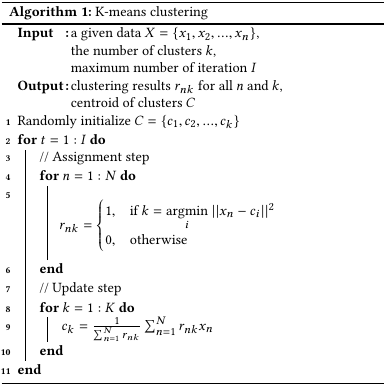
\includegraphics[width=200pt]{5.png} 
    \caption{k-means clustering 알고리즘} 
    \label{fig:3} 
\end{figure}

\section{Related Works}
빅데이터 분석은 현재 코로나를 비롯하여 다양한 분야에서 이용되고있다. 서울시에서 관리하는 빅데이터 분석 연합에서는 다양한 공모전을 비롯하여 아이디어와 빅데이터를 이용하여 생활에 편의가 되도록 노력하고 있다.

그 중 대표적인 것이 서울 및 경기도 지역의 시간대별 자전거 이동량을 조사하여 자전거 거치소의 설치가 필요한 지역이지만, 아직 자전거 거치소가 설치되어 있지 않은 지역을 파악하고, 자전거 거치소를 설치하는 제안을 하였다. 시간대별로 인구의 유동성을 나누어서 분석한 점은 시간대별로 유동인구가 차이를 보이고, 유동인구가 많은 지역과 적은 지역이 다를 것이라는 아이디어를 얻을 수 있었다.

다만 너무 세분화시켜서 지역을 구분한 탓에 방역을 하는데 있어서는 그냥 전체 지역을 하는것과 똑같은 결과를 얻을 수 밖에없었고, 
거점 지역을 기준으로하여 좀 더 큰 사이즈로 유동성이 큰 지역을 찾기위하여 k-means Clustering을 이용하였다.

또한 현재 코로나에 대한 빅데이터가 가장 많이 이루어지는 분야는 확진자의 이동 시간대와, 이동 동선을 이용하여 밀접접촉자를 찾고 빠른 검사를 통해 확진자가 더 생겨나지않게하는 확진자 수의 감소에 많은 관심이 있는 편이다. 그리고 이에 따라 지역 전체에 걸쳐 강화된 방역을하고 하기때문에 경제적으로나, 환경적으로 비효율적일 수 밖에없다. 이를 해결하기 위해 시간대별로 효율적인 방역을 위한 지역과 방역구역선택을 하는데 있어 DBSCAN과 k-means Clustering을 이용하여 중심 지역으로 선택하였다.

\section{My idea}
T-Drive trajectory data sample는 2008년도에 베이징시의 택시 이동경로를 분석한 데이터이므로 코로나와는 무관한 시기이기 때문에, 현 시기라 가정한다. 또한, 택시로 이동한 사람들을 베이징시의 유동인구로써 가정한다.

처음으로 택시 데이터를 시간대에 따라서 DBSCAN을통해 분류하였다. 이 이유는 시간대마다 유동인구가 밀집되는 지역이 다를 것이라 예상하고 시간대에 따라서 특정 지역의 방역강도를 정한 뒤 단계에 따라 방역하고, 또한 단계에 따라 주민들에게 재난 경고 문자 등을 발송하여 바이러스가 퍼지는 것을 막을 수 있다.

이렇게 시간대로 나누어 가장 유동성이 높은 시간대는 장소에 상관없이 최고단계의 방역을 실시하고, 사람이 밀집되는 곳이니 피해달라고 문자를 발송할 수 있다. 이제 나머지 시간대는 크게 출근, 점심, 퇴근 후 휴식시간으로 시간대를 나누어 준다.

유동성이 최고인 시간대를 제외한 나머지 시간대에는 베이징시 전체가 유동성이 높은 것이 아니라 특정지역이 유동성이 높을 것이라고 예상하고 각 시간대 내에서 유동 인구수를 기준으로, 많은 지역들을 클러스터링을 통해 확인하여 각 지역에 유동성에 비례하여 방역의 단계를 정하여 효율적이고 경제적으로 방역을 진행할 수 있다. 
 
\section{The Details}
처음 결과는 시간대 분류를 통하여 유동성이 젤 높은 시간대를 찾았다.
위 그래프는 x축(시간대), y축(유동 인구수, 100만단위)으로 나타낸 것이다. 빨간색은 시간대에 속한 유동 인구수를 의미하고 파란색은 전체에 따른 비율을 의미한다. 그래프에서 보면 알 수 있듯이 14:00~18:00시간대에 비율이 압도적으로 높은 것을 확인할 수 있다. 이 시간대에는 지역에 상관없이 전체에 걸쳐 유동인구수가 많다는 것을 의미하므로 베이징시의 전역에 대해 최고 단계의 방역을 시행하고, 불필요한 외출 삼가를 바라는 재난 문자를 국민들에게 보내어 바이러스의 확산을 막을 수 있을 것이다.

이제 나머지 시간대 새벽 시간  (02:00~06:00), 출근시간(06:00~10:00), 점심시간(10:00~14:00), 퇴근/유흥시간(18:00~22:00) 에 대하여 각각의 유동 인구수를 클러스터링을 통해 지역별로 묶어 주었다. 
\begin{figure}[htp] 
    \centering
    
\includegraphics[width=120pt]{6.png} 
    \caption{제안 방법의 알고리즘} 
    \label{fig:4} 
\end{figure}

\begin{figure*}[htp] 
    \centering
    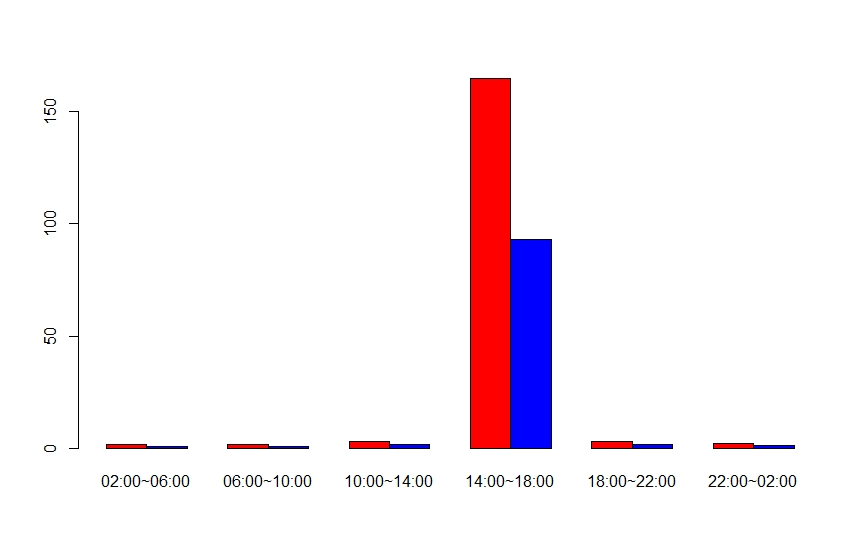
\includegraphics[width=\textwidth]{2.jpg} 
    \caption{시간대별 유동 인구수} 
    \label{fig:5} 
\end{figure*}

\begin{figure*}[htp] 
    \centering
    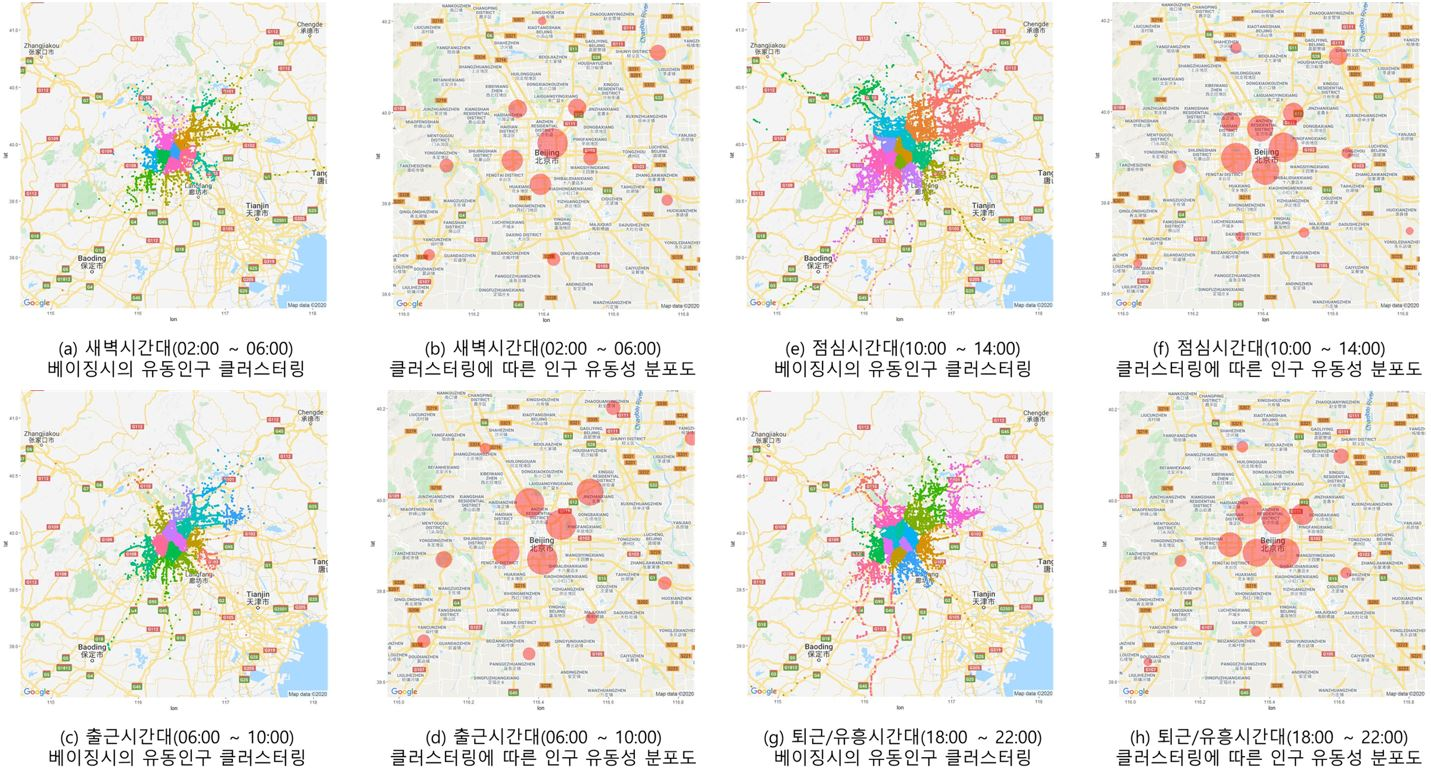
\includegraphics[width=\textwidth]{7.jpg} 
    \caption{시간대별 인구의 유동성 클러스터링 및 분포도} 
    \label{fig:6} 
\end{figure*}

이 때 클러스터 된 개수가 많으면 많을수록 원의 크기를 크게 하였고, 클러스터 된 수가 적다면 분포도에서 제거하여 주었다. 새벽 시간대의 분포도를 보면 유동인구가 집중되는 지역이 출근시간대와 다르게 베이징시를 중심으로 하여 오각형의 형태를 이루는 것을 볼 수 있다. 또한 원의 크기가 중심부는 크고 주위 지역은 작은 것을 볼 수 있다. 이 뜻은 새벽시간대에는 중심부가 외곽지역에 비해 유동인구수가 많고, 외곽지역은 유동인구수가 적다는 것을 의미한다. 따라서 방역을 해주는데 있어서, 새벽시간대에는 중심부지역의 방역단계를 높게 하고, 외곽 지역의 방역단계는 상대적으로 낮게 하여서 효율적으로 방역을 할 수 있을 것이다.

출근시간대와 점심시간대의 유동성 분포도를 보면, 원의 크기와 분포 형태는 비슷하나, 원이 생성된 지점이 다른 것을 볼 수 있다. 이 말은 인구의 이동지역과 수가 비슷하긴 하지만, 위치에 있어 조금씩 차이가 있다는 것을 의미하고, 방역을 중점적으로 해야 할 위치에 대해 차이가 생긴다는 것을 의미한다. 마지막으로 퇴근 및 유흥시간대의 데이터를 보면, 확연히 원의 크기와 분포형태가 다른 시간대와 차이를 보이는 것을 볼 수 있다. 또한 원의 크기 역시 대부분 큰 원들로 구성되어 있는 것으로 보아 유동인구수도 많다는 것을 의미한다. 이 시간대에는 아까 유동인구가 최고 시간대인 14:00~18:00 시간대와 비슷하게 중심지역들을 기준으로 하여 철저한 방역을 하는 것이 좋을 것이다.

한 가지 눈에 들어오는 점은 베이징시 최 외곽 지역에도 인구 유동성이 어느정도 인 지역들이 있다. 이러한 지역들은 간과되어 질 수 있는데, 데이터를 통해, 이러한 지역들 역시 간과하지 않고, 낮은 방역단계를 통해서라도, 방역이 이루어진다면, 좀 더 확실하게 바이러스의 확산을 차단하는데 도움이 될 것이다. 이러한 결과들을 통해 만약 이러한 데이터 분석이 없다면, 아마 방역을 하는데 있어서 어느 정도 수준으로 해야 할지 정하지못할 것이고, 어느 지역이 인구 유동성이 많은지도 파악하지 못할 것이다.

따라서 방역을 하는데 있어 여러 인건비와 방역재료비 등에 대해서 비효율적인 상황이 나올 것이고, 또한 최 외곽지역은 유동 인구수가 기준 이상임에도 불구하고 멀다는 이유로 무시되거나 하는 제대로 된 방역이 이루어 지지 않을 수 있다. 시간대별 지역 클러스터링과 분포도를 통하여 효율적인 방역이 가능하고, 주민들에게 현재 시간대에 대해서 인구 유동성이 높은 지역과 낮은 지역에 대한 알람을 통해 위험 지역을 피하게 하는 등 여러 대책을 보다 편하게 세울 수 있을 것이다.

\section{Conclusions and futher work}
본 보고서에서는 장기화되고 있는 코로나19 바이러스 감염을 효과적으로 통제 관리하기 위해 T-Drive trajectory 데이터를 Database scan을 이용하여 데이터를 분류한 뒤 k means clustering 알고리즘을 사용하여, 시민들이 많이 군집하는 지역의 시간대별 통행 및 혼잡 패턴을 분석했다.

시민들이 주로 군집하는 장소의 정보를 이용하여 효과적인 방역 지점을 선정 및 운용하고, 시민의 안전을 도모하고 불편을 최소화할 수 있는 안전 통행 경로와 관련 교통 운영정책을 효과적으로 수립 및 운용하는데 도움이 될 것이다. 추가적으로 데이터를 운용할 때, 택시에 대한 정보 뿐 아니라 버스나 지하철 같은 일반 대중들이 더 자주 이용하는 대중교통의 데이터를 이용한다면 결과에 대한 정확성을 더 높일 수 있을 것 이다.

또 추가적으로 감염자들의 통행 이력을 직접적으로 사용한다면 관련 접촉자들을 신속하게 파악할 수 있을 것이고, 방역 당국 및 감염 접촉자들에게 신속하게 전달함으로써, 바이러스의 확산을 효과적으로 예방할 수 있을 것이다. 하지만 이러한 데이터들은 개인의 사생활을 침해한다는 논란이 있어 개인정보활용에 대한 문제를 극복하는 것이 수반되어야 할 것이다.

\ifCLASSOPTIONcaptionsoff
  \newpage
\fi

\begin{thebibliography}{1}
\bibitem{IEEEhowto:kopka}
H.~Kopka and P.~W. Daly, \emph{A Guide to \LaTeX}, 3rd~ed.\hskip 1em plus
  0.5em minus 0.4em\relax Harlow, England: Addison-Wesley, 1999.
\bibitem{IEEEhowto:kopka}
Wagstaff, K., Cardie, C., Rogers, S., & Schrödl, S. (2001, June). Constrained k-means clustering with background knowledge. In Icml (Vol. 1, pp. 577-584).
\bibitem{IEEEhowto:kopka}
Likas, Aristidis, Nikos Vlassis, and Jakob J. Verbeek. "The global k-means clustering algorithm." Pattern recognition 36.2 (2003): 451-461.
\bibitem{IEEEhowto:kopka}
Bradley, P. S., & Fayyad, U. M. (1998, July). Refining initial points for k-means clustering. In ICML (Vol. 98, pp. 91-99).
\bibitem{IEEEhowto:kopka}
Alsabti, K., Ranka, S., & Singh, V. (1997). An efficient k-means clustering algorithm.
\bibitem{IEEEhowto:kopka}
Kanungo, T., Mount, D. M., Netanyahu, N. S., Piatko, C. D., Silverman, R., & Wu, A. Y. (2002). An efficient k-means clustering algorithm: Analysis and implementation. IEEE transactions on pattern analysis and machine intelligence, 24(7), 881-892.
\bibitem{IEEEhowto:kopka}
Bradley, P. S., Bennett, K. P., & Demiriz, A. (2000). Constrained k-means clustering. Microsoft Research, Redmond, 20(0), 0.
\bibitem{IEEEhowto:kopka}
김남순. "코로나바이러스감염증-19 현황과 과제." 보건· 복지 Issue & Focus 373 (2020): 1-13.
\bibitem{IEEEhowto:kopka}
이한나, 김유휘, 김진희, 오다은, 이정은, 이주연, ... & 최요석. (2020). 코로나바이러스감염증-19 확산에 대한 방문돌봄서비스의 대응 및 과제. 보건· 복지 Issue & Focus, 378, 1-11.
\bibitem{IEEEhowto:kopka}
박준범. (2020). 정책논단: 코로나 바이러스 감염병 2019 와 보건정책. The KAPS, 60, 8-11.
\bibitem{IEEEhowto:kopka}
현정희, 김정현, 이혜영, 곽진, 김자은, 이은영, ... & 김한숙. (2020). 코로나바이러스감염증-19 1 번 환자 접촉자 조사 결과. 주간 건강과 질병, 13(7), 352-358.
\bibitem{IEEEhowto:kopka}
현정희, 이정현, 박영준, & 정은경. (2020). 한국 초기 코로나바이러스감염증-19 환자 28 명의 역학적 특성. 주간 건강과 질병, 13(9), 464-474.
\bibitem{IEEEhowto:kopka}
웹사이트, http://ncov.mohw.go.kr/
\bibitem{IEEEhowto:kopka}
오효정, 윤보현, 최남현, 유철중, & 김용. (2014). 소셜 빅데이터 내용 분석 기반 사용자 그룹별 선호지역 및 이동패턴 시각화. 한국정보기술학회논문지, 12(12), 195-203.
\bibitem{IEEEhowto:kopka}
구자용. (2017). 공간 빅 데이터를 이용한 개인 활동패턴의 시공간적 탐색: 서울시 지역의 트윗 데이터를 사례로. 국토지리학회지, 51(3), 259-270.
\bibitem{IEEEhowto:kopka}
임종태, 복경수, & 유재수. (2019). 빅데이터 분석 기법을 이용한 실시간 대중교통 경로 안내 시스템의 설계 및 구현. 한국콘텐츠학회논문지, 19(2), 460-468.
\bibitem{IEEEhowto:kopka}
이종용, 정계동, 류기환, & 박세영. 빅 데이터를 활용한 의정부 지역 관광 분석 연구. The Journal of the Convergence on Culture Technology (JCCT), 6(1), 413-418.
\bibitem{IEEEhowto:kopka}
임종태, 김기연, 김재구, 오현교, 윤수용, 박선용, ... & 유재수. (2014). 빅데이터 분석을 통한 실시간 최적 교통 경로 안내 시스템의 설계 및 구현. 한국콘텐츠학회 종합학술대회 논문집, 297-298.
\bibitem{IEEEhowto:kopka}
Shin, J. E., Oh, Y. S., & Lim, D. H. (2016). RHadoop platform for K-Means clustering of big data. Journal of the Korean Data and Information Science Society, 27(3), 609-619.
\bibitem{IEEEhowto:kopka}
Song, J., & Lee, S. M. (2015). A Study on the Application Modeling of SNS Big-data for a Micro-Targeting using K-Means Clustering. In Proceedings of the Korean Society of Computer Information Conference (pp. 321-324). Korean Society of Computer Information.
\bibitem{IEEEhowto:kopka}
Kwon, S., Kim, S., Tak, O., & Jeong, H. (2017). A Study on the Clustering Method of Row and Multiplex Housing in Seoul Using K-Means Clustering Algorithm and Hedonic Model. Journal of Intelligence and Information Systems, 23(3), 95-118.
\bibitem{IEEEhowto:kopka}
Jung, S. H., Shin, C. S., Cho, Y. Y., Park, J. W., Park, M. H., Kim, Y. H., ... & Sim, C. B. (2017). Analysis Process based on Modify K-means for Efficiency Improvement of Electric power Data Pattern Detection. Journal of Korea Multimedia Society, 20(12), 1960-1969.
\bibitem{IEEEhowto:kopka}
송용욱. (2019). 내비게이션 빅데이터를 활용한 시간대별 통행패턴 분석 (Doctoral dissertation, 한양대학교).
이수현, 정영선, & 김재윤. (2014). K-means 클러스터링의 타당성 검증을 위한 새로운 유효성 지수. 한국경영학회 통합학술발표논문집, 492-507.
\bibitem{IEEEhowto:kopka}
이재구, 이태훈, & 윤성로. (2014). Big Data 분석을 위한 Machine Learning. 한국통신학회지 (정보와통신), 31(11), 14-26.
\bibitem{IEEEhowto:kopka}
Sim, G. S., Kim, Y. H., Lee, J. H., Kim, J. H., & Park, Y. J. (2014). 빅 데이터 분석을 위한 맵리듀스 알고리즘의 최근 연구 동향. Communications of the Korean Institute of Information Scientists and Engineers, 32(1), 27-32.
\bibitem{IEEEhowto:kopka}
유건화, & 황철수. (2019). 도시 연구를 위한 시, 공간 클러스터링: 비모수적 접근. 대한지리학회 학술대회논문집, 45-45.
\bibitem{IEEEhowto:kopka}
김민석, 최우성, & 정순영. (2018). 알고리즘 시각화 기반 클러스터 분석 학습 시스템 설계 및 구현. 한국정보과학회 학술발표논문집, 933-935.
\bibitem{IEEEhowto:kopka}
서영원, & 김창수. (2015). 맵리듀스 기반 DFP-Tree 를 이용한 클러스터링 알고리즘. 인터넷정보학회논문지, 16(6), 23-30.
\bibitem{IEEEhowto:kopka}
이태민, 최우성, & 정순영. (2015). Parallel K-Means 학습을 위한 시뮬레이터 설계 및 개발. 한국컴퓨터교육학회 학술발표대회논문집, 19(1), 101-105.
\bibitem{IEEEhowto:kopka}
Kim, K. I., & Kim, J. S. (2019). Big Data Processing and Performance Improvement for Ship Trajectory using MapReduce Technique. 한국컴퓨터정보학회논문지, 24(10), 65-70.
\bibitem{IEEEhowto:kopka}
강성민, 이석주, & 민준기. (2015). 맵리듀스를 이용한 다중 중심점 집합 기반의 효율적인 클러스터링 방법. 정보과학회 컴퓨팅의 실제 논문지, 21(7), 494-499.
\bibitem{IEEEhowto:kopka}
Yun, U., Ryang, H., Lee, G., & Fujita, H. (2017). An efficient algorithm for mining high utility patterns from incremental databases with one database scan. Knowledge-Based Systems, 124, 188-206.
\bibitem{IEEEhowto:kopka}
Kulldorff, M., Fang, Z., & Walsh, S. J. (2003). A tree‐based scan statistic for database disease surveillance. Biometrics, 59(2), 323-331.
\bibitem{IEEEhowto:kopka}
Chakraborty, S., Nagwani, N. K., & Dey, L. (2014). Performance comparison of incremental k-means and incremental dbscan algorithms. arXiv preprint arXiv:1406.4751.
\bibitem{IEEEhowto:kopka}
Mumtaz, K., & Duraiswamy, K. (2010). A novel density based improved k-means clustering algorithm–Dbkmeans. International Journal on computer science and Engineering, 2(2), 213-218.
\bibitem{IEEEhowto:kopka}
Smiti, A., & Elouedi, Z. (2012, June). Dbscan-gm: An improved clustering method based on gaussian means and dbscan techniques. In 2012 IEEE 16th international conference on intelligent engineering systems (INES) (pp. 573-578). IEEE.
\bibitem{IEEEhowto:kopka}
Erman, J., Arlitt, M., & Mahanti, A. (2006, September). Traffic classification using clustering algorithms. In Proceedings of the 2006 SIGCOMM workshop on Mining network data (pp. 281-286).
\bibitem{IEEEhowto:kopka}
Dudik, J. M., Kurosu, A., Coyle, J. L., & Sejdić, E. (2015). A comparative analysis of DBSCAN, K-means, and quadratic variation algorithms for automatic identification of swallows from swallowing accelerometry signals. Computers in biology and medicine, 59, 10-18.
\bibitem{IEEEhowto:kopka}
Edla, D. R., Jana, P. K., & Member, I. S. (2012). A prototype-based modified DBSCAN for gene clustering. Procedia Technology, 6, 485-492.
\bibitem{IEEEhowto:kopka}
Verma, M., Srivastava, M., Chack, N., Diswar, A. K., & Gupta, N. (2012). A comparative study of various clustering algorithms in data mining. International Journal of Engineering Research and Applications (IJERA), 2(3), 1379-1384.
\bibitem{IEEEhowto:kopka}
Kanagala, H. K., & Krishnaiah, V. J. R. (2016, January). A comparative study of K-means, DBSCAN and OPTICS. In 2016 International Conference on Computer Communication and Informatics (ICCCI) (pp. 1-6). IEEE.
\bibitem{IEEEhowto:kopka}
Bandyopadhyay, S. K., & Paul, T. U. (2013). Segmentation of brain tumour from mri image analysis of k-means and dbscan clustering. International Journal of Research in Engineering and Science, 1(1), 48-57.
\bibitem{IEEEhowto:kopka}
Viswanath, P., & Pinkesh, R. (2006, August). l-dbscan: A fast hybrid density based clustering method. In 18th International Conference on Pattern Recognition (ICPR'06) (Vol. 1, pp. 912-915). IEEE.
\bibitem{IEEEhowto:kopka}
Shen, J., Hao, X., Liang, Z., Liu, Y., Wang, W., & Shao, L. (2016). Real-time superpixel segmentation by DBSCAN clustering algorithm. IEEE transactions on image processing, 25(12), 5933-5942.
\bibitem{IEEEhowto:kopka}
Bai, Y., Yao, L., Wei, T., Tian, F., Jin, D. Y., Chen, L., & Wang, M. (2020). Presumed asymptomatic carrier transmission of COVID-19. Jama, 323(14), 1406-1407.
\bibitem{IEEEhowto:kopka}
Zu, Z. Y., Jiang, M. D., Xu, P. P., Chen, W., Ni, Q. Q., Lu, G. M., & Zhang, L. J. (2020). Coronavirus disease 2019 (COVID-19): a perspective from China. Radiology, 200490.
\bibitem{IEEEhowto:kopka}
Tian, S., Hu, N., Lou, J., Chen, K., Kang, X., Xiang, Z., ... & Chen, G. (2020). Characteristics of COVID-19 infection in Beijing. Journal of Infection.


\end{thebibliography}




\begin{IEEEbiographynophoto}{Cheol Woo Park}
Cheol Woo Park received the B.S. degree
in physics from Pusan National University,
South Korea, in 2018, where he is currently pursuing
the M.S. degree in electronics engineering.
His research interests include computer vision and
image processing.

\end{IEEEbiographynophoto}

\begin{IEEEbiographynophoto}{Jun Young Park}
Jun Young Park received the B.S. degree
in electronic engineering from Pusan National University,
South Korea, in 2017, where he is currently pursuing
the M.S. degree in electronics engineering.
His research interests include computer vision and
image processing.
\end{IEEEbiographynophoto}

\end{document}